%!TEX root = main.tex

\section*{Exercises}
\begin{problem}[Advanced]
State and prove similar statements as in Definition \ref{def:localminimum}, Theorems \ref{theorem:localminimum}, \ref{theorem:2DTforLEV} and \ref{theorem:MaxMinCompact}, but for \emph{local} and \emph{global maxima}.
\end{problem}

\begin{problem}[Basic]
Find and sketch the domain of the following functions.
\begin{enumerate}
	\item $f(x,y) = \sqrt{y-x-2}$
	\item $f(x,y) = \log \big( x^2+y^2-4 \big)$
	\item $f(x,y) = \frac{(x-1)(y+2)}{(y-x)(y-x^3)}$
	\item $f(x,y) = \log (xy+x-y-1)$
\end{enumerate}
\end{problem}

\begin{problem}[Basic]
Find and sketch the level lines $f(x,y)=c$ on the same set of coordinate axes for the given values of $c$.
\begin{enumerate}
	\item $f(x,y) = x+y-1$, $c \in \{ -3, -2, -1, 0, 1, 2, 3\}$.
	\item $f(x,y) = x^2+y^2$, $c \in \{ 0, 1, 4, 9, 16, 25 \}$.
	\item $f(x,y) = xy$, $c \in \{ -9, -4, -1, 0, 1, 4, 9 \}$
\end{enumerate}
\end{problem}

\begin{problem}[CAS]\label{problem:countours}
Use a Computer Algebra System of your choice to produce contour plots of the given functions on the given domains.
\begin{enumerate}
	\item $f(x,y) = (\cos x)(\cos y) e^{-\sqrt{x^2+y^2}/4}$ on $[-2\pi, 2\pi]\times [-2\pi, 2\pi]$.
	\item $g(x,y) = \dfrac{xy(x^2-y^2)}{x^2+y^2}$ on $[-1,1] \times [-1,1]$
	\item $h(x,y) = y^2 - y^4 -x^2$ on $[-1,1]\times[-1,1]$
	\item $k(x,y) = e^{-y}\cos x$ on $[-2\pi, 2\pi]\times[-2,0]$
\end{enumerate}
\begin{figure}[ht!]
\begin{tabular}{cc}
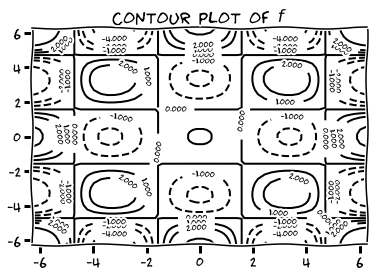
\includegraphics[width=0.5\linewidth]{images/contourf.png} &
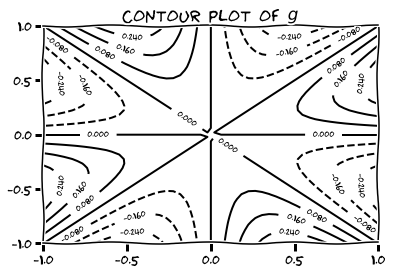
\includegraphics[width=0.5\linewidth]{images/contourg.png} \\
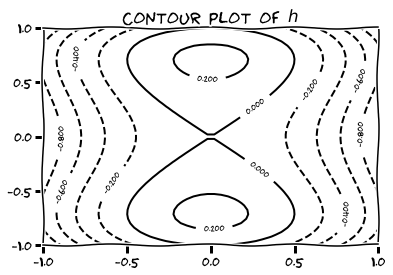
\includegraphics[width=0.5\linewidth]{images/contourh.png} &
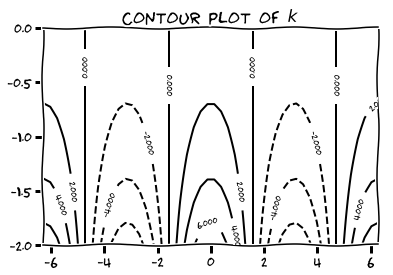
\includegraphics[width=0.5\linewidth]{images/contourk.png} 
\end{tabular}
\caption{Contour plots for problem \ref{problem:countours}}
\end{figure}
\end{problem}

\begin{problem}[Basic]
Sketch the curve $f(x,y)=c$ together with $\gradient{f}$ and the tangent line at the given point.  Write an equation for the tangent line.
\begin{enumerate}
	\item $f(x,y)=x^2+y^2$, $c=4$, $(\sqrt{2}, \sqrt{2})$.
	\item $f(x,y)=x^2-y$, $c=1$, $(\sqrt{2}, 1)$.
	\item $f(x,y)=xy$, $c=-1$, $(2, -1/2)$.
	\item $f(x,y)=x^2-xy+y^2$, $c=7$, $(-1,2)$.
\end{enumerate}
\end{problem}

\begin{problem}[Basic]
For the function
\begin{equation*}
f(x,y) = \frac{x-y}{x+y},
\end{equation*}
at the point $P_0 = (-1/2, 3/2)$, find the directions $\boldsymbol{v}$ and the directional derivatives $D_{\boldsymbol{v}}f(P_0)$ for which
\begin{enumerate}
	\item $D_{\boldsymbol{v}}f(P_0)$ is largest.
	\item $D_{\boldsymbol{v}}f(P_0)$ is smallest.
	\item $D_{\boldsymbol{v}}f(P_0) = 0$.
	\item $D_{\boldsymbol{v}}f(P_0) = 1$.
	\item $D_{\boldsymbol{v}}f(P_0) = -2$.
\end{enumerate}
\end{problem}

\begin{problem}[Intermediate]
The derivative of $f(x,y)$ at $(1,2)$ in the direction $\frac{\sqrt{2}}{2}[1,1]$ is $2\sqrt{2}$ and in the direction $[0,-1]$ is $-3$.  What is the derivative of $f$ in the direction $\frac{\sqrt{5}}{5}[-1,-2]$?
\end{problem}

\begin{problem}[Intermediate]
Find the absolute maxima and minima of the function $f(x,y) = (4x-x^2)\cos y$ on the rectangular plate $1\leq x \leq 3, -\frac{\pi}{4} \leq y \leq \frac{\pi}{4}$.
\end{problem}

\begin{problem}[Basic]
Find two numbers $a \leq b$ such that 
\begin{equation*}
\int_a^b (24-2x-x^2)^{1/3}\, dx
\end{equation*}
has its largest value.
\end{problem}

\begin{problem}[Basic] % example 2, p.858 in Thomas' Calculus
Find the points of the hyperbolic cylinder $x^2-z^2-1=0$ in $\field{R}^3$ that are closest to the origin.
\end{problem}

\begin{problem}[Intermediate]
Find the extreme values of the function $f(x,y,z)=xy+z^2$ on the circle in which the plane $y-x=0$ intersects the sphere $x^2+y^2+z^2=4$.
\end{problem}

\begin{problem}[CAS]
Write a routine (in your favorite CAS) that uses \emph{symbolic computation}\footnote{See Appendix \ref{appendix:sympy}} to find the minimum of a differentiable real-valued function $f \colon \field{R} \to \field{R}$ over 
\begin{enumerate}
	\item a closed interval $[a,b]$
	\item An interval of the form $[a,\infty)$, or $(-\infty, b]$
\end{enumerate}
The routine should accept as input:
\begin{itemize}
	\item the expression of the function $f$,
	\item the endpoints $a,b$.
\end{itemize}
\end{problem}